\chapter{Metodologia}
A arquitetura do sistema Robinho foi projetada utilizando a linguagem AADL desde as fases iniciais do desenvolvimento. Essa abordagem baseada em modelos permitiu que decisões arquiteturais fossem tomadas com base em análises rigorosas, visando maximizar eficiência, confiabilidade e determinismo temporal do sistema embarcado.
O processo de modelagem seguiu uma abordagem iterativa e incremental. Inicialmente, foram definidos o fluxo de dados, os dispositivos físicos envolvidos e os comportamentos esperados do sistema. A partir dessa visão funcional, os componentes foram formalmente descritos em AADL, incluindo sensores, atuadores, unidades de processamento e os aplicações de \textit{software} responsáveis pela orquestração das funcionalidades.

De acordo com a figura tal, blablabla TODO

\begin{figure}[htbp]
\begin{center}
    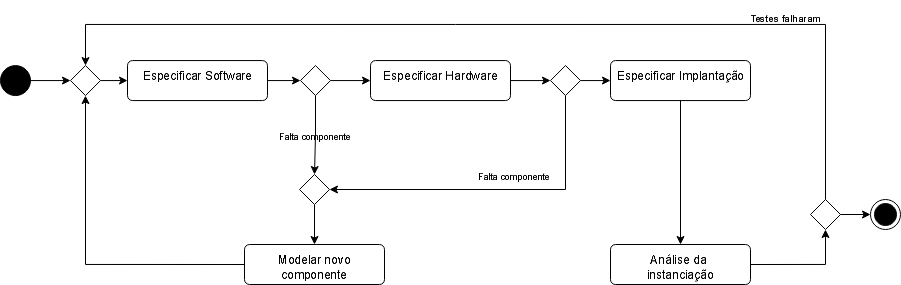
\includegraphics[width=\linewidth]{images/fluxo trabalho.png}
    \caption{Fluxo de trabalho de modelagem}\vspace{-0.5cm}
\end{center}
\end{figure}

como evidencia a figura, etc

Os componentes foram organizados em uma hierarquia modular de pacotes, projetada para promover reutilização, clareza e manutenibilidade. Cada pacote agrupa elementos logicamente relacionados, como subsistemas de controle, interfaces de sensoriamento, processamento de visão e controle de mobilidade. No modelo de Robinho, por exemplo, o sistema de tração diferencial e o módulo ESP-CAM   foram representados como dispositivos independentes, enquanto a unidade central de processamento foi modelada como um sistema contendo múltiplos processos e threads que integram dados de sensores e geram comandos de atuação.

Após a definição da estrutura lógica, os próximos passos envolvem alimentar o modelo com propriedades relacionadas a performance, que permitem análises formais de escalonabilidade e uso de recursos por meio da ferramenta OSATE:

\begin{itemize}
    \item MIPSBudget - Carga de um processo em MIPS.
    \item Compute\_Execution\_Time - Tempo de execução de um processo.
    \item Period - Período da execução de um processo.
    \item MIPSCapacity - Capacidade de um processador em MIPS.
    \item RAMCapacity - Capacidade de RAM de uma memória.
    \item BandwidthCapacity - Capacidade de banda de um barramento.
    \item DataSize - Tamanho de uma informação transmitida.
\end{itemize}

Com o modelo completamente especificado, é feita sua instanciação. Esta etapa permite a  validação para consistência arquitetural, corretude de fluxo de dados e restrições temporais. No caso de Robinho, isto inclui verificar se a imagem consegue ser processada e transmitida dentro do tempo limite para gerar comandos de movimento com latência mínima e máxima eficiência.

Finalmente, depois de o modelo ser instanciado, o OSATE permite o uso das ferramentas de análise integradas, como análise de latência, simulação de escalonamento e previsão de uso de recursos, para definir se a arquitetura atual cumpre os requisitos do sistema. Caso quaisquer gargalos ou violações sejam detectadas, o modelo pode ser refinado iterativamente, suportando uma metodologia de design antes da implementação, que reduz significativamente os riscos de integração durante a implantação.

Repetidas vezes durante o processo de modelagem, foram encontrados gargalos computacionais e na comunicação entre os componentes. Nestes casos, O uso dos componentes específicos e meios de comunicação foi reavaliado, e iterativamente os componentes do sistema foram avaliados, e se necessário, alterados.

Um dos principais benefícios da abordagem centrada em modelos foi a capacidade de evoluir o sistema sem comprometer a validade da arquitetura. Quando módulos de software foram substituídos ou novas funcionalidades foram incorporadas, bastou modelar os novos componentes e reexecutar as análises, sem necessidade de reformular toda a arquitetura ou refazer validações previamente concluídas.

Essa metodologia de projeto dirigido por modelos permitiu que decisões arquiteturais fossem documentadas, quantitativamente validadas e refinadas muito antes da integração física, reduzindo drasticamente riscos

Como resultado, a implantação do sistema em hardware real ocorreu com alta confiança de que os requisitos não funcionais seriam atendidos desde a primeira inicialização.